%!TEX TS-program = xelatex
\documentclass[]{friggeri-cv}
\usepackage{afterpage}
\usepackage{hyperref}
\usepackage{url}
\usepackage{color}
\usepackage{xcolor}
\hypersetup{
    pdftitle={herve.beraud.cv.en.pdf},
    pdfauthor={herve beraud},
    pdfsubject={Hervé Beraud curriculum vitae},
    pdfkeywords={},
    colorlinks=false,       % no lik border color
   allbordercolors=white    % white border color for all
}
\addbibresource{bibliography.bib}
\RequirePackage{xcolor}
\definecolor{pblue}{HTML}{0395DE}

\begin{document}
\header{Hervé }{Beraud}
      {Python Software Engineer}
      
% Fake text to add separator      
\fcolorbox{white}{gray}{\parbox{\dimexpr\textwidth-2\fboxsep-2\fboxrule}{%
.....
}}

% In the aside, each new line forces a line break
\begin{aside}
  \section{Address}
    Rue~Longuebrune~d'astarac
    32450,~Castelnau~Barbarens,~France
    ~
  \section{Tel}
    +33 661 840 417
    ~
  \section{Mail}
    \href{mailto:herve.beraud@openmailbox.org}{\textbf{herve.beraud@}\\openmailbox.org}
    ~
  \section{Web \& Git}
    \href{http://hberaud.tilola.com}{hberaud.tilola.com}
    \href{https://github.com/4383}{github.com/4383}
    ~
  \section{Programming}
    
\includegraphics[scale=0.15]{img/programming.png}
    ~
  \section{OS Preference}
    \textbf{GNU/Linux}
\includegraphics[scale=0.40]{img/5stars.png}
    \textbf{Unix}
\includegraphics[scale=0.40]{img/4stars.png}
    \textbf{MacOS}
\includegraphics[scale=0.40]{img/2stars.png}
    \textbf{Windows}
\includegraphics[scale=0.40]{img/1stars.png}
    ~
  \section{Personal Skills}
    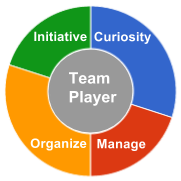
\includegraphics[scale=0.62]{img/personal.png}
    ~
\end{aside}

\section{Experience}
\begin{entrylist}
  \entry
    {04/14 - Now}
    {Software Engineer}
    {BULL / EDF, Toulouse, France}
    {Design and development of algorithms, solutions for call center and workload management system. Design and development of multi-channel agent desktop.\\}
  \entry
    {09/13 - 03/14}
    {Embedded Software Engineer}
    {BULL / French Navy, Aix en Provence, France}
    {Design continuous integration, Design system architecture , AIX5.3 and Unix software.\\}
    \entry
    {02/13 - 09/13}
    {Software Engineer}
    {BULL / DCNS, Toulon, France}
    {Design, development electronic warefare system on the FREMM frigate project.\\}
    \entry
    {06/11 - 01/13}
    {Frontend / Backend Web Developer}
    {BULL / Virtual-expo, Marseille, France}
    {Design, development of an world expert online exhibitions website on Linux/Apache/PHP/Zend platform. Design, development of an Python web crawler.\\}
    \entry
    {04/11 - 06/11}
    {System Administrator / Backend Developer}
    {Distrimag, Arles, France}
    {Maintain data center environmental and monitoring equipment (IBM AS400). Virtualize physical server. PHP Development of stock managment software.\\}
    \entry
    {10/10 - 03/11}
    {Frontend Web / Backend Developer}
    {PlusValue SAS, Vitrolles, France}
    {Management and migration of servers. Development php web micro-framework. Development of web templates and interfaces. Management of SQL databases.\\}
    \entry
    {12/04 - 01/09}
    {Buisness Owner}
    {Damofli Fruits \& Legumes, France}
    {Manage marketing operations, accounting, sales plans, inventory management.\\}
    \entry
    {09/01 - 11/04}
    {Landscape Architect}
    {Local Council of Martigues, France}
    {Manage marketing operations, accounting, sales plans, inventory management.}
\end{entrylist}

\newpage
\section{Education}
\begin{entrylist}
  \entry
    {2010 - Now}
    {Master's Degree in Computer Engineering}
    {CNAM Aix en Provence, France}
    {Curriculum informations systems.\\
    Main subjects: Systems \& Software Architecture and Security, Urbanism for evolving systems.\\}
  \entry
    {2009 - 2010}
    {BTEC Higher National Diploma in Software Development}
    {AFPA Istres, France}
    {Main subjects: Software Architectire, modeling tools (Merise, UML).\\}
  \entry
    {1999 - 2001}
    {BTEC National Diploma in Landscape Architect}
    {Lycée Fontlongue Miramas, France}
    {Agricultural college.\\
    Main subjects: Design and Advise on the construction of urban, rural, residential and public landscape.\\}
  \entry
    {1999 - 2001}
    {BTEC First Diploma in Nursery Gardener}
    {Lycée Fontlongue Miramas, France}
    {Agricultural college.\\
    Main subjects: cultivating, harvesting, transplanting trees, shrubs or plants.}
\end{entrylist}

\section{Realisations and Personal projects}
\begin{entrylist}
  \entry
    {11-2014}
    {www.tilola.com}
    {Personal project}
    {\emph{Python 3 / Django 1.7 / Nginx / Tastypie / Gunicorn / PostGreSQL / Debian 7}}
  \entry
    {07/2014}
    {garage-denavaux.fr}
    {Personal project}
    {\emph{Python / Bottle / Gunicorn / Nginx / Debian 7}}
  \entry
    {02/2013}
    {github.com/4383/fabric-debian/}
    {Personal project}
    {\emph{Python / Iptables /  debian 6 / port-knocking / Fail2Ban / PostGreSQL / Nginx}}
  \entry
    {2012}
    {medical-expo.com}
    {Virtual-expo.com project}
    {\emph{PHP5.3 / Apache 2 / Mysql 5}}
  \entry
    {10/2012}
    {github.com/4383/battle-story/}
    {Personal project}
    {\emph{Python / Pygame}}
  \entry
    {09/2012}
    {github.com/4383/WebForge/}
    {Personal project}
    {\emph{Python / Tkinter}}
  \entry
    {2010}
    {http://fr.wikipedia.org/wiki/Neo\_Keyboard}
    {Personal project}
    {\emph{C / C++ / SDL}}
  \entry
    {2010}
    {http://fr.wikipedia.org/wiki/Metronomix}
    {Personal project}
    {\emph{C / C++ / SDL}}
\end{entrylist}


\begin{aside}
~
~
~
  \section{Places Lived}
    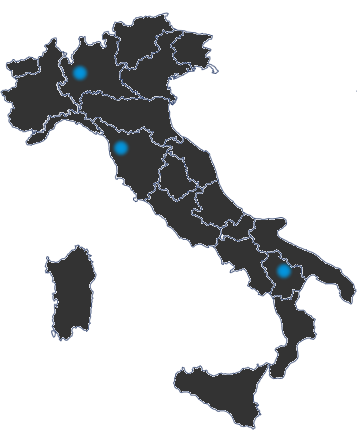
\includegraphics[scale=0.25]{img/italia.png}
    ~
  \section{About me}
    Year of birth : 1982
    married, 3 childrens 
    ~
  \section{Languages}
    \textbf{French}
\includegraphics[scale=0.40]{img/5stars.png}
    \textbf{English}
\includegraphics[scale=0.40]{img/3stars.png}
\end{aside}

\section{Hobbies and Interests}
\begin {itemize}
    \item \emph {Sports (Crossfit, Swinmming, Running)}
    \item \emph {Family}
    \item \emph {Programming (ArchLinux, Python, Arduino, Vim)}
    \item \emph {Traveling (Senegal, Ivory Coast, Europe)}
\end {itemize}

~
\begin{flushleft}
\emph{November 20th, 2014}
\end{flushleft}
\begin{flushright}
\emph{Hervé Beraud}
\end{flushright}


\end{document}
